\section{Arquitectura SCV}
\frame
{
\frametitle{Arquitectura SCV centralizado}
\begin{itemize}
 \item Todo el mundo actualiza un mismo repositorio central remoto
 \item La gestión de ramas y tags es más una convención que parte de la herramienta
\end{itemize}

\begin{center}
 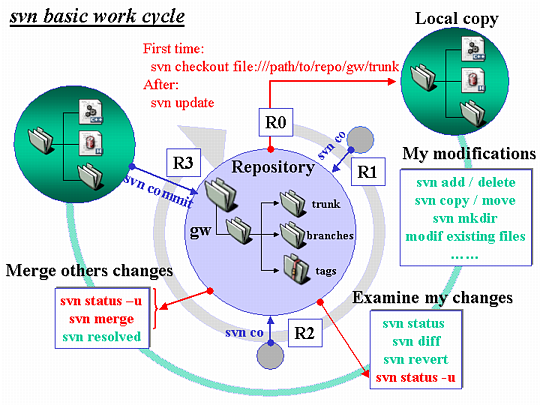
\includegraphics[height=5cm]{imgs/svnscheme.png}
\end{center}
}

\frame
{
\frametitle{Arquitectura SCV distribuido}
\begin{itemize}
 \item Todo el mundo mantiene su copia del proyecto
 \item Cada integrante del equipo trabaja en sus propias funcionalidades en su repositorio local particular
 \item El mantenedor del repositorio acepta o no las modificaciones de los integrantes
\end{itemize}

\begin{center}
 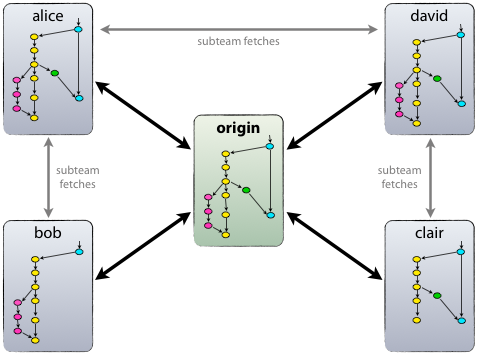
\includegraphics[height=5cm]{imgs/gitscheme.png}
\end{center}
}

\frame
{
\frametitle{GIT}
\begin{itemize}
 \item Nacido de la mente de Linus Torvalds. Versión 1.0 en 2005. 
\end{itemize}

\begin{center}
  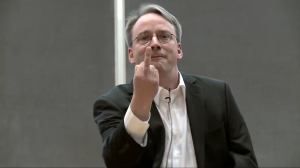
\includegraphics[height=2cm]{imgs/linus.png}    
\end{center}

\begin{itemize}
 \item Se buscaba una manera de gestionar la ingente cantidad de código del kernel de Linux
 \item Toma el diseño de versiones anteriores de BitKeeper y Monotone
 \item Git se basa en \textit{snapshots}, cada commit es una copia completa del código comprimida en binario, lo que le imprime velocidad. Usan compresión delta zlib para optimizar el espacio.
 \item Se ha medido git log frente a svn log, git opera 100x más rápido
 \item Se opera siempre en local (de ahí el incremento de velocidad) y cuando se tienen listos los cambios se suben a remoto
\end{itemize}
}